\chapter{Situation de départ - Programme dans la carte d'évaluation (DSP)}

\section{Introduction}
Ce chapitre a pour but de présenter l'architecture logicielle développée lors du précédent projet de Bachelor par Thomas Freyche \cite{Freyche}.

\section{Principe du fonctionnement du programme}
Le fichier principal \texttt{hrpwm\_ex1\_duty\_sfo.c} a été développé pour assurer la sustentation du démonstrateur. Ce programme étant dense, il ne sera pas présenté dans son intégralité. Seules les portions de code considérées comme structurantes seront détaillées.

Ce fichier centralise l'ensemble de la logique de commande, particulièrement la régulation, l'acquisition des données ADC et la communication sans fil. Les fonctionnalités implémentées sont les suivantes :

\begin{itemize}
    \item Gestion des interruptions.
    \item Lecture de 8 canaux ADC (mesures de position et de courant par inducteur).
    \item Conversion des valeurs brutes de l'ADC en grandeurs physiques.
    \item Procédure de lancement de la sustentation.
    \item Régulation de position par retour d'état.
    \item Régulation de courant par le biais de régulateurs PI.
    \item Calcul des rapports cycliques (PWM) générés par les boucles de régulation.
    \item Affectation des signaux PWM aux broches de commande des ponts en H.
    \item Communication UART avec le module ESP32.
\end{itemize}

\section{Algorithme du code principal}
\label{sec:Algo}
Actuellement, l'algorithme du programme principal respecte l'organigramme suivant :

\begin{figure}[H]
    \centering
    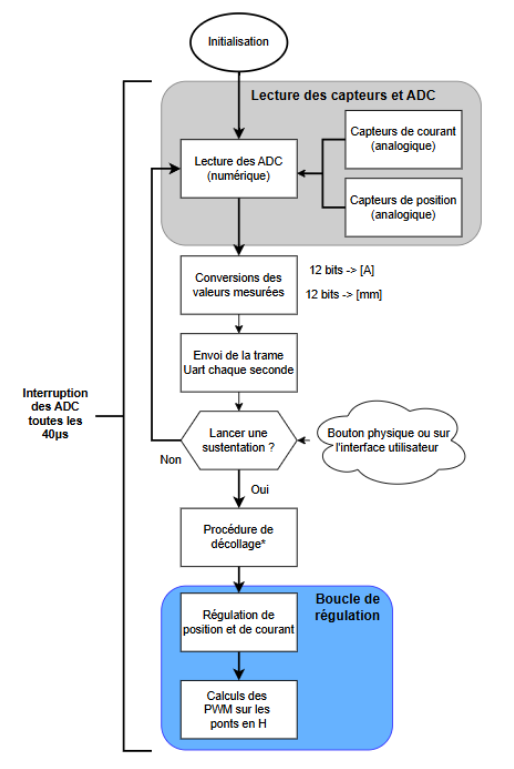
\includegraphics[width=0.7\linewidth]{assets/content/03-CodePrincipale/Algorithme.png}
    \caption{Structure de l'algorithme du code principal \cite{Freyche}}
    \label{fig:AlgorithmeCodePrincipal}
\end{figure}

La majeure partie du code s'exécute au sein d'une routine d'interruption. Celle-ci englobe l'acquisition et la conversion des valeurs ADC, l'exécution des algorithmes de régulation, la mise à jour des modules PWM ainsi que la gestion de l'interface utilisateur (boutons).

\section{Éléments principaux du programme}
Le programme principal étant dense, seuls les éléments considérés comme importants seront présentés.

\subsection{Bibliothèques}
Le projet s'appuie sur les dépendances suivantes :

\begin{minted}{c}
#include "driverlib.h"
#include "device.h"
#include "board.h"
#include "sfo_v8.h"
#include "math.h"
#include "stdio.h"
#include "FunctionHeader.h"
\end{minted}

\begin{itemize}
    \item \texttt{driverlib.h} : Bibliothèque fondamentale du DSP TI C2000. Elle met à disposition des fonctions de haut niveau permettant la configuration matérielle (ex. : \texttt{ADC\_readResult}, \texttt{GPIO\_writePin}) en s'affranchissant de la manipulation directe des registres.
    \item \texttt{device.h} : Fichier de configuration spécifique au microcontrôleur utilisé. Il définit les fonctions d'initialisation système requises pour le fonctionnement de l'horloge et des périphériques.
    \item \texttt{board.h} : Fichier généré par l'outil SysConfig (voir \autoref{subsubsec:SysConfig}). Il regroupe les définitions des entrées/sorties paramétrées via l'interface graphique.
    \item \texttt{sfo\_v8.h} : Bibliothèque indispensable pour l'exploitation de la fonctionnalité HRPWM (High-Resolution PWM). Elle assure une calibration continue des signaux afin de compenser les dérives thermiques et les fluctuations de tension.
    \item \texttt{math.h} et \texttt{stdio.h} : Bibliothèques standards C dédiées aux calculs mathématiques et à la gestion des flux d'entrées/sorties.
    \item \texttt{FunctionHeader.h} : Fichier d'en-tête local regroupant les définitions paramétriques spécifiques à la maquette (détaillé dans la \autoref{subsubsec:FunctionHeader}).
\end{itemize}

\subsubsection{SysConfig}
\label{subsubsec:SysConfig}
L'outil SysConfig, exploité au travers du fichier \texttt{hrpwm\_ex1\_duty\_sfo.syscfg}, offre une interface de configuration graphique du DSP. Son utilisation permet d'initialiser les modules suivants :

\begin{itemize}
    \item Les convertisseurs analogiques-numériques (ADC).
    \item Les générateurs de signaux PWM.
    \item Le module de communication série SCI (UART).
\end{itemize}

L'interface propose une vue schématique du microcontrôleur simplifiant l'affectation des broches (pin mapping). Lors de la validation de cette configuration, l'outil génère automatiquement les fichiers sources \texttt{board.h} et \texttt{board.c}.

\subsubsection{\texttt{FunctionHeader.h}}
\label{subsubsec:FunctionHeader}
Ce fichier regroupe l'ensemble des définitions de constantes et des prototypes de fonctions exploités dans le projet. Les éléments qui y sont définis incluent :

\begin{itemize}
    \item Les paramètres physiques : caractéristiques mécaniques et électromagnétiques de la maquette (entrefer nominal, masse, inductance et géométrie des bobines).
    \item Les configurations électriques : tension du bus continu (48~V) et résolution de quantification de l'ADC (12~bits).
    \item Les paramètres PWM : fréquence de découpage (25~kHz), gestion des temps morts (dead bands) des MOSFET et corrections temporelles associées.
    \item Les paramètres de la régulation de courant (PI) : seuil de courant au décollage (3~A), ainsi que les paramètres de régulation $K_p$, $\tau_i$ et $G_i$.
    \item Les paramètres de la régulation de position (Espace d'état) : coefficients de rétroaction $K_\omega$, $K_d$ et $K_r$.
    \item Les filtres numériques : dimensionnement des fenêtres et coefficients propres aux filtres IIR, FIR et de Savitzky-Golay.
\end{itemize}

\subsection{Fonctions principales}

\subsubsection{La fonction \texttt{PI\_current\_regulator}}
L'implémentation de la fonction \texttt{PI\_current\_regulator} se présente ainsi :

\begin{minted}{c}
void PI_current_regulator(float ic, float current, float *integral,
float *ue, float *uc){
    float ie = (ic - current) * KP_I;
    *integral += (ie - *ue) * GI_I * H;
    float uc_prim = ie + *integral;

    *uc = uc_prim;
    if (uc_prim > UMAX) {
        *uc = UMAX;
    }
    if (uc_prim < 0) {
        *uc = 0;
    }

    *ue = (uc_prim - *uc) * ANTIWINDUP_EN;
}
\end{minted}

Cette fonction assure la régulation du courant au moyen d'une structure PI. Les arguments qui lui sont passés sont :

\begin{itemize}
    \item La consigne de courant \texttt{ic}.
    \item Le courant réel mesuré \texttt{current}.
    \item Le pointeur de la variable d'intégration \texttt{integral}.
    \item Le pointeur de l'erreur de tension \texttt{ue}.
    \item Le pointeur de la tension de commande calculée \texttt{uc}.
\end{itemize}

La séquence de régulation s'articule selon les étapes suivantes :

\begin{enumerate}
    \item Calcul de l'erreur $i_e$ (différence entre la consigne et la mesure du courant), puis multiplication par le gain proportionnel.
    \item Mise à jour de l'action intégrale par sommation de la différence entre l'erreur de courant $i_e$ et l'erreur de tension $u_e$, pondérée par le gain intégral $GI_I$ et la période d'échantillonnage $H$.
    \item Évaluation de la commande intermédiaire $u_{c\_prim}$, obtenue par la somme des actions proportionnelle et intégrale.
    \item Limitation de la commande (saturation) afin de respecter les limites physiques imposées par l'alimentation de la maquette (plage de 0~V à $U_{MAX} = 48$~V). La consigne finale est restreinte à ces bornes le cas échéant.
    \item Calcul de l'écart de tension (différence entre la commande intermédiaire et la commande limitée) pondéré par le coefficient d'anti-windup, afin de prévenir l'emballement de l'intégrateur.
\end{enumerate}

Cette fonction est appelée de manière cyclique dans la routine d'interruption principale pour assurer l'asservissement en courant des quatre bobines.

\subsubsection{Filtre de Savitzky-Golay}
\label{subsubsec:Savitzky}
Le code du filtre de Savitzky-Golay est implémenté de la façon suivante :

\begin{minted}{c}
float savitzky_Filter(float *Buffer)
{
    float v = 0.0f;
    uint16_t m = 0;

    for(m = 0; m < FILTWINDOW; m++)
        v += F_PWM*Buffer[m]*SAVITZKY[m];

    for(m = 0; m < FILTWINDOW-1; m++)
        Buffer[m] = Buffer[(m+1)];

    return v;
}
\end{minted}

Ce filtre \cite{Savitzky} est utilisé pour lisser les mesures fortement bruitées tout en conservant au mieux la dynamique temporelle du signal utile.

Le principe de fonctionnement est illustré par la \autoref{fig:PrincipeSavitzky} :

\begin{figure}[H]
    \centering
    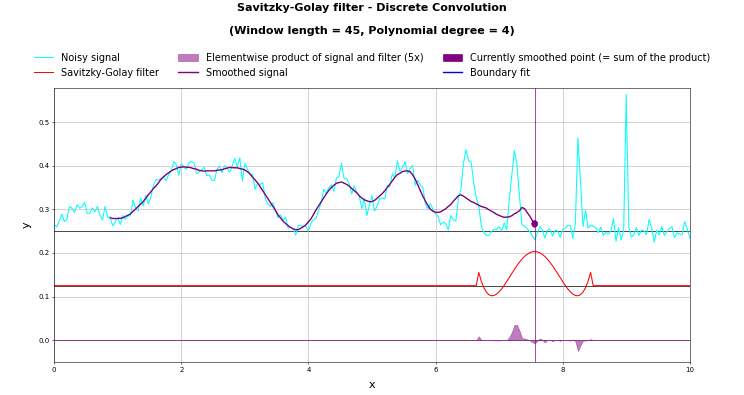
\includegraphics[width=1\linewidth]{assets/content/03-CodePrincipale/PrincipeSyvitzky.png}
    \caption{Principe de lissage du filtre de Savitzky-Golay \cite{Savitzky}}
    \label{fig:PrincipeSavitzky}
\end{figure}

Le traitement s'apparente à l'application d'un filtre FIR à fenêtre glissante. Dans son paramétrage actuel, la fonction mémorise les neuf dernières acquisitions de position. Une somme pondérée est calculée en multipliant chaque échantillon par un coefficient propre au filtre de Savitzky-Golay :

\begin{minted}{c}
//savitzky filter coefficients, order = 2, window = 9
const float SAVITZKY[FILTWINDOW] = {-0.0667, -0.05, -0.0333, -0.0167,
                                     0.0, 0.0167, 0.0333, 0.05, 0.0667};
\end{minted}

L'élargissement de la fenêtre glissante permet d'améliorer l'atténuation du bruit, mais ce lissage introduit un retard dans la réponse du système. Ce filtre est spécifiquement implémenté dans le firmware pour dériver la position et en filtrer le résultat afin d'obtenir la vitesse :

\begin{minted}{c}
        // --- Filtres de vitesse Savitzky-Golay ---
        pos1Buff[FILTWINDOW-1] = Position1;
        v1 = savitzky_Filter(pos1Buff);

        pos2Buff[FILTWINDOW-1] = Position2;
        v2 = savitzky_Filter(pos2Buff);

        pos3Buff[FILTWINDOW-1] = Position3;
        v3 = savitzky_Filter(pos3Buff);

        pos4Buff[FILTWINDOW-1] = Position4;
        v4 = savitzky_Filter(pos4Buff);
\end{minted}

\subsubsection{Filtre coupe-bande}
L'algorithme du filtre coupe-bande est rédigé comme suit :

\begin{minted}{c}
float IIR_Filter(float *entree, float *sortie)
{
    float somme = 0.0;
    float somme2 = 0.0;

    uint16_t k = 0;

    //difference equation
    for(k = 0; k < Nb; k++) //Num.
        somme += b[k]*entree[k];
    for(k = 0; k < Na; k++) //Den.
        somme2 += a[k]*sortie[k];

    //update buffers
    for(k = (Na-1); k > 0; k--)
        sortie[k] = sortie[(k-1)];

    sortie[0] = (somme-somme2);

    for(k = (Nb-1); k > 0; k--)
        entree[k] = entree[(k-1)];

    return (somme-somme2);
}
\end{minted}

Ce filtre est synthétisé sous la forme d'un filtre IIR. Son rôle consiste à atténuer une perturbation de résonance observée autour de 75~Hz. Si l'origine physique précise de cette oscillation reste à ce jour inexpliquée, son atténuation est une condition stricte pour maintenir la stabilité des boucles de régulation.\\

Les coefficients paramétrés sont les suivants :

\begin{minted}{c}
    //bandstop Filter 75Hz 2nd order bande coupe de 40Hz  130Hz (6)
#define A1_B1_6         -1.977307757140243538
#define A2_6            0.97763254912161579
#define B0_B2_6         0.98881627456080789517756
\end{minted}

\subsubsection{La fonction \texttt{SendFloatAsText}}
La fonction \texttt{SendFloatAsText} permet la transmission des données de position vers l'interface web. Elle est définie comme suit :

\begin{minted}{c}
    void SendFloatAsText(float f0, float f1, float f2, float f3)
    {
        char str[TX_BUF_LEN];
        int i = 0, j = 0;

    // Mise en forme de la trame envoyée
        str[i++] = '\x02'; // start bit

        i += ftoa(f0, &str[i], 3);
        str[i++] = ',';

        i += ftoa(f1, &str[i], 3);
        str[i++] = ',';

        i += ftoa(f2, &str[i], 3);
        str[i++] = ',';

        i += ftoa(f3, &str[i], 3);

        str[i++] = '\x03'; // stop bit

        for (j = 0; j < i && j < TX_BUF_LEN; j++) {
            txBuffer[j] = (uint8_t)str[j];
        }

        txLength = i;
        txIndex = 0;

        // Envoi de la trame
        SCI_enableInterrupt(SCIA_BASE, SCI_INT_TXFF);
    }
\end{minted}

Cette fonction récupère quatre variables puis les envoie à l'ESP32, qui s'occupe de l'affichage.

\section{Les interruptions}
Le programme possède plusieurs interruptions. La principale, dénommée \texttt{adcA1ISR}, exécute l'algorithme du programme. Cette interruption correspond donc à l'algorithme de base décrit dans l'\autoref{sec:Algo}.

Les deux autres interruptions sont employées pour la communication UART entre la carte d'évaluation et l'ESP32. La transmission permet, comme expliqué précédemment, d'envoyer les données à l'ESP32. Celle-ci se décrit comme suit :

\begin{minted}{c}
    // --- UART Transmit (TX) ---
    __interrupt void INT_mySCI0_TX_ISR(void)
    {
        while (SCI_getTxFIFOStatus(SCIA_BASE) < SCI_FIFO_TX16 && txIndex < txLength)
        {
            SCI_writeCharBlockingFIFO(SCIA_BASE, txBuffer[txIndex++]);
        }

        if (txIndex >= txLength)
        {
            SCI_disableInterrupt(mySCI0_BASE, SCI_INT_TXFF); // Fin d'envoi
        }

        SCI_clearOverflowStatus(SCIA_BASE);
        SCI_clearInterruptStatus(SCIA_BASE, SCI_INT_TXFF);
        Interrupt_clearACKGroup(INTERRUPT_ACK_GROUP9);
    }
\end{minted}

La réception est principalement employée pour recevoir l'état d'activation du système. La maquette peut ainsi être activée à distance depuis l'interface web. L'interruption de réception est décrite comme suit :

\begin{minted}{c}
    // --- UART Receive (RX) ---
    __interrupt void INT_mySCI0_RX_ISR(void)
    {
        uint16_t c;
        int b;

        while (SCI_getRxFIFOStatus(SCIA_BASE) > 0)
        {
            c = SCI_readCharBlockingFIFO(SCIA_BASE);
            if (rxIndex < RX_BUF_LEN) {
                rxBuffer[rxIndex++] = c;
            }

            if(c == '\x02'){
                dataIndex = rxIndex; // Début de trame
            }

            if(c == '\x03'){ // Fin de trame
                if(dataIndex > 0 && dataIndex < rxIndex - 1) {
                    // Utilisation d'une évaluation booléenne directe !
                    state_PIN = (rxBuffer[dataIndex] == '1');
                }
                // Reset du buffer
                rxIndex = 0;
                for(b = 0; b < RX_BUF_LEN; b++) {
                    rxBuffer[b] = 0;
                }
            }
        }

        SCI_clearOverflowStatus(SCIA_BASE);
        SCI_clearInterruptStatus(SCIA_BASE, SCI_INT_RXFF);
        Interrupt_clearACKGroup(INTERRUPT_ACK_GROUP9);
    }
\end{minted}